\documentclass[12pt,notitle,letterpaper]{report}
% generated by Docutils <http://docutils.sourceforge.net/>
% rubber: set program xelatex
\usepackage{fontspec}
% \defaultfontfeatures{Scale=MatchLowercase}
% straight double quotes (defined T1 but missing in TU):
\ifdefined \UnicodeEncodingName
  \DeclareTextCommand{\textquotedbl}{\UnicodeEncodingName}{%
    {\addfontfeatures{RawFeature=-tlig,Mapping=}\char34}}%
\fi
\usepackage{ifthen}
\usepackage{alltt}
\usepackage{amsmath}
\usepackage{graphicx}
\usepackage{longtable,ltcaption,array}
\setlength{\extrarowheight}{2pt}
\newlength{\DUtablewidth} % internal use in tables

%%% Custom LaTeX preamble
% Linux Libertine (free, wide coverage, not only for Linux)
\setmainfont{Linux Libertine O}
\setsansfont{Linux Biolinum O}
\setmonofont[HyphenChar=None,Scale=MatchLowercase]{DejaVu Sans Mono}

%%% User specified packages and stylesheets
% embedded stylesheet: c:\Users\rodhh\Dropbox\projects\residence_remodel\rivtcalcs0001\docs\d00\pdf_style.sty
\makeatletter
%%
%% default LaTex report class style for rivtcalc 
%%
\usepackage{lastpage}
\usepackage{fancyhdr}
\usepackage{titlesec}
\usepackage{fontspec}
\usepackage{dejavu}
\usepackage{bm}
\usepackage{gensymb}
\usepackage[normalem]{ulem}
\usepackage{etoolbox}
\usepackage{tabulary}
\usepackage{geometry}
\usepackage{mathastext}
%% font size
\setmainfont{DejaVu Sans}[Scale=0.8]
\setsansfont{DejaVu Sans}[Scale=0.8]
\setmonofont{DejaVu Sans Mono}[Scale=0.8]
\setmathrm{Arial}
\setmathsf{Arial}
\setmathtt{Arial}
\DeclareMathSizes{10}
\renewcommand\familydefault\sfdefault
%% \usepackage[libertine]{newtxmath}

%% margins
\geometry{hmargin={0.5in,0.5in},vmargin={0.8in,0.8in}}
\setlength{\parindent}{0in}
\setlength{\parskip}{.1in}
\renewenvironment{quote}
  {\small\list{}{\rightmargin=0cm \leftmargin=0cm}%
   \item\relax}
  {\endlist}
%% pagestyle plain - table of contents
%% header
\pagestyle{fancy}
\fancyhf{}
\fancyhead[L]{\normalsize  Carport Wind Model}
\fancyhead[R]{\normalsize c0303 | \thepage}
\renewcommand\chaptermark[1]{\markboth{#1}{}} 
\renewcommand\sectionmark[1]{\markright{\thesection.\ #1}}
%% footer
\fancyfoot[C]{calc file: \jobname .py \hfill \today\ }
\renewcommand\headrulewidth{1pt}
\renewcommand\footrulewidth{1pt}
%% modify section headings - chapters
\titleformat{\chapter}
 [display]
 {\normalfont\large\bfseries}
 {}{0pt}
 {\large}
 [\vspace{2mm}\titlerule]
\titlespacing*{\chapter}{0pt}{-40pt}{12pt}
%% modify section headings - sections
\titleformat{\section}
 [display]
 {\normalfont\large\bfseries}
 {}{0pt}
 {\large}
 [\vspace{2mm}\titlerule]
\titlespacing*{\section}{0pt}{-40pt}{12pt}


\makeatother

%%% Fallback definitions for Docutils-specific commands

% transition (break, fancybreak, anonymous section)
\providecommand*{\DUtransition}{%
  \hspace*{\fill}\hrulefill\hspace*{\fill}
  \vskip 0.5\baselineskip
}
% hyperlinks:
\ifthenelse{\isundefined{\hypersetup}}{
  \usepackage[colorlinks=true,linkcolor=blue,urlcolor=blue]{hyperref}
  \usepackage{bookmark}
  \urlstyle{same} % normal text font (alternatives: tt, rm, sf)
}{}


%%% Body
\begin{document}
\setcounter{page}{1}


\vspace{.2in}   \textbf{Carport Unit Loads and Weight}   \hfill\textbf{SECTION 01}
\newline   \vspace{.05in}   {\color{black}\hrulefill}

\textbf{Roof unit dead loads} \hfill  {[}Table: 0303.01{]}

\setlength{\DUtablewidth}{\linewidth}
\begin{longtable*}[c]{|p{0.133\DUtablewidth}|p{0.098\DUtablewidth}|p{0.121\DUtablewidth}|p{0.400\DUtablewidth}|}
\hline
\textbf{%
variable
} & \textbf{%
value
} & \textbf{%
{[}value{]}
} & \textbf{%
description
} \\
\hline
\endfirsthead
\hline
\textbf{%
variable
} & \textbf{%
value
} & \textbf{%
{[}value{]}
} & \textbf{%
description
} \\
\hline
\endhead
\multicolumn{4}{c}{\hfill ... continued on next page} \\
\endfoot
\endlastfoot

ld1
 & 
2.0 psf
 & 
0.096 KPa
 & 
Urethane foam (4 inch thick)
 \\
\hline

ld2
 & 
1.0 psf
 & 
0.048 KPa
 & 
Three-ply roofing
 \\
\hline

ld3
 & 
5.0 psf
 & 
0.239 KPa
 & 
Doug Fir decking 2-in.
 \\
\hline

ld4
 & 
1.0 psf
 & 
0.048 KPa
 & 
Doug Fir beams 4x12 at 12 ft o.c.
 \\
\hline
\end{longtable*}

\textbf{Carport Geometry} \hfill  {[}Table: 0303.02{]}

\begin{quote}
\begin{alltt}
==========  ===========  ==========  ===============
variable          value     [value]  description
==========  ===========  ==========  ===============
cp_width     22.75 [ft]    6.93 [m]  carport width
cp_length     19.5 [ft]    5.94 [m]  carport length
roofdl1     0.009 [ksf]  0.43 [KPa]  unit load
newfnd      0.15 [kips]   0.67 [KN]  new foundations
==========  ===========  ==========  ===============
\end{alltt}
\end{quote}

\textbf{Weight of carport} \hfill {[} Equ: 0303.01{]}
%
\begin{equation*}
cp_{wt} = cp_{length} \cdot cp_{width} \cdot roofdl_{1} + 6 \cdot newfnd
\end{equation*}
\begin{quote}
\begin{alltt}
=========================  ===========  ===========  ==========  ==========
          cp_wt              newfnd      cp_length    cp_width    roofdl1
=========================  ===========  ===========  ==========  ==========
4.89 [kips]  [21.76 [KN]]  0.15 [kips]  19.50 [ft]   22.75 [ft]  0.01 [ksf]
=========================  ===========  ===========  ==========  ==========
\end{alltt}
\end{quote}

\vspace{.2in}   \textbf{Wind loads}   \hfill\textbf{SECTION 02}
\newline   \vspace{.05in}   {\color{black}\hrulefill}

\textbf{Wind Force Values} \hfill  {[}Table: 0303.03{]}

\begin{quote}
\begin{alltt}
==========  ==========  ==========  ===========================
variable         value     [value]  description
==========  ==========  ==========  ===========================
uplift_max  2.8 [kips]  12.46 [KN]  nominal maximum wind uplift
==========  ==========  ==========  ===========================
\end{alltt}
\end{quote}

\textbf{Uplift DC ratio} \hfill {[} Equ: 0303.02{]}
%
\begin{equation*}
dc_{1} = \frac{uplift_{max}}{0.9 \cdot cp_{wt}}
\end{equation*}
\begin{quote}
\begin{alltt}
====================  ============  ===========
        dc1            uplift_max      cp_wt
====================  ============  ===========
0.64 [-]  [0.64 [-]]  2.80 [kips]   4.89 [kips]
====================  ============  ===========
\end{alltt}
\end{quote}

\textbf{Mecca Wind Model Results} \hfill  {[}Table: 0303.04{]}

\begin{quote}
\begin{alltt}
**MecaWind v2374**

    Software Developer: Meca Enterprises Inc., [www.meca.biz](http://www.meca.biz/), Copyright © 2020



    Calculations Prepared by:                    Calculations Prepared For:
    StL                                           Client:      Bryna Holland
    15 Blanca Drive                               Project #:           00120
    Novato, California, 94947                     Location:    Mill Valley, California
    Date: Feb 10, 2021                            Description:
    Designer: rholland                            Residential Remodel



    File Location : F:\textbackslash{}Dropbox\textbackslash{}projects\textbackslash{}residence_remodel\textbackslash{}models\textbackslash{}MecaWind\textbackslash{}carport1.wnd



**Basic Wind Parameters**

    Wind Load Standard           = ASCE 7-16       Exposure Category            = B
    Wind Design Speed            = 100.0 mph       Risk Category                = III
    Structure Type               = Building        Building Type                = Open



**General Wind Settings**

    Incl_LF   = Include ASD Load Factor of 0.6 in Pressures                     = True
    DynType   = Dynamic Type of Structure                                       = Rigid
    NF        = Natural Frequency of Structure (Mode 1)                         = 1.000 Hz
    Zg        = Altitude (Ground Elevation) above Sea Level                     = 0.000 ft
    Bdist     = Base Elevation of Structure                                     = 0.000 ft
    SDB       = Simple Diaphragm Building                                       = False
    Reacs     = Show the Base Reactions in the output                           = True
    MWFRSType = MWFRS Method Selected                                           = Ch 27 Pt 1



**Topographic Factor per Fig 26.8-1**

    Topo      = Topographic Feature                                             = None
    Kzt       = Topographic Factor                                              = 1.000



**Building Inputs**

    RoofType: Roof Type          = MonoSlope       h       : Mean Roof Height   = 8.000 ft
    L       : Width Normal to Ridge= 19.000 ft     D       : Length Along Ridge = 23.000 ft
    WindFlow: Wind Flow Method   = Clear           Slope   : Slope of Roof      = 5.0 Deg
    Frames  : Incl Transverse Frames= False        n       : Number of Frames   = 3
    e       : Solidity Ratio     = 0.100



**Exposure Constants per Table 26.11-1:**

    Alpha: Table 26.11-1 Const   = 7.000           Zg:    Table 26.11-1 Const   = 1200.000 ft
    At:    Table 26.11-1 Const   = 0.143           Bt:    Table 26.11-1 Const   = 0.840
    Am:    Table 26.11-1 Const   = 0.250           Bm:    Table 26.11-1 Const   = 0.450
    C:     Table 26.11-1 Const   = 0.300           Eps:   Table 26.11-1 Const   = 0.333



**Gust Factor Calculation:**

    Gust Factor Category I Rigid Structures - Simplified Method
    G1        = For Rigid Structures (Nat. Freq.>1 Hz) use 0.85                 = 0.85
    Gust Factor Category II Rigid Structures - Complete Analysis
    Zm        = 0.6 * Ht                                                        = 30.000 ft
    Izm       = Cc * (33 / Zm) ^ 0.167                                          = 0.305
    Lzm       = L * (Zm / 33) ^ Epsilon                                         = 309.993
    Q         = (1 / (1 + 0.63 * ((B + Ht) / Lzm)^0.63))^0.5                    = 0.906
    G2        = 0.925*((1+1.7*lzm*3.4*Q)/(1+1.7*3.4*lzm))                       = 0.869
    Gust Factor Used in Analysis
    G         = Lessor Of G1 Or G2                                              = 0.850



**Main Wind Force Resisting System (MWFRS) Calculations per Ch 27 Part 1:**

    LF        = Load Factor based upon ASD Design                               = 0.60
    h         = Mean Roof Height above grade                                    = 8.000 ft
    Kh        = Z < 15 ft [4.572 m]--> (2.01 * (15/zg)^(2/Alpha) \{Table 26.10-1\}= 0.575
    Kzt       = Topographic Factor is 1 since no Topographic feature specified  = 1.000
    Kd        = Wind Directionality Factor per Table 26.6-1                     = 0.85
    qh        = (0.00256 * Kh * Kzt * Kd * Ke * V^2) * LF                       = 7.50 psf



**Wind Pressures on Open Building Monoslope Free Roof per Fig 27.4.4 - Wind
Dir 0 Deg:**


style="COLOR: rgb(0,0,255); TEXT-ALIGN: center"> **MWFRS Pressures per Fig
27.3-4 on Monoslope Free Roof - Wind Dir 0 Deg**

**All wind pressures include a load factor of 0.6**



          Load Case             Cnw              Cnl              Pnw             Pnl
                                                                  psf             psf
         -----------           ------           ------           -----           -----
         Load Case A            1.200            0.300            7.65            1.91
         Load Case B           -1.100           -0.100           -7.02           -0.64



       Notes:
       Pnw   = Pressure on windward portion of roof:  qh*G*Cnw*LF    \{Eqn 27.3-4\}
       Pnl   = Pressure On Leeward portion Of roof:   qh*G*Cnl*LF    [Eqn 27.3-4]
       All wind pressures include a load factor of 0.6
       + Pressures Acting TOWARD Surface          - Pressures Acting AWAY from Surface



**Reactions Roof +GCPi Wind Dir 0 Deg**



          Description    Pressure    Area     Fx     Fy      Fz      Mx       My      Mz
                           psf        ft     Kip    Kip     Kip     k-ft     k-ft    k-ft
         -------------   --------   ------   ----   ----    ----    -----    ----    ----
         Leeward Roof        1.91   219.33   0.00   0.04    0.42     1.71    0.00    0.00
         Windward Roof       7.65   219.33   0.00   0.15    1.67    -9.17    0.00    0.00
         -------------   --------   ------   ----   ----    ----    -----    ----    ----
         Total               0.00   438.67   0.00   0.18    2.09    -7.47    0.00    0.00



**Reactions Roof -GCPi Wind Dir 0 Deg**



          Description    Pressure    Area     Fx     Fy      Fz      Mx       My      Mz
                           psf        ft     Kip     Kip     Kip    k-ft     k-ft    k-ft
         -------------   --------   ------   ----   -----   -----   -----    ----    ----
         Leeward Roof       -0.64   219.33   0.00   -0.01   -0.14   -0.57    0.00    0.00
         Windward Roof      -7.02   219.33   0.00   -0.13   -1.53    8.41    0.00    0.00
         -------------   --------   ------   ----   -----   -----   -----    ----    ----
         Total               0.00   438.67   0.00   -0.15   -1.67    7.84    0.00    0.00



**Wind Pressures on Open Building Monoslope Free Roof per Fig 27.4.7 - Wind
Dir 90 Deg:**


style="COLOR: rgb(0,0,255); TEXT-ALIGN: center"> **Open Building Along Ridge
Pressures per Fig 27.3-7 - Wind 90 Deg**

**All wind pressures include a load factor of 0.6**



         Roof Var     Start       End        CnA         CnB       Pressure      Pressure
                       Dist       Dist                               PnA           PnB
                        ft         ft                                psf           psf
         --------     ------     ------     ------      -----      --------      --------
         Roof_1        0.000      8.000     -0.800      0.800         -5.10          5.10
         Roof_2        8.000     16.000     -0.600      0.500         -3.83          3.19
         Roof_3       16.000     23.000     -0.300      0.300         -1.91          1.91



         Notes Roof Pressures:
         Start Dist = Start Dist from Windward Edge  End Dist = End Dist from Windward Edge
         CnA        = Cn for Load Case A             CnB      = Cn for Load Case B
         PnA        = qh*G*CnA \{Eqn 27.4-3\}          PnB      = qh*g*CnB  \{Eqn 27.4-3]
         + Pressures Acting TOWARD Surface          - Pressures Acting AWAY from Surface




**Reactions Roof +GCPi Wind Dir 90 Deg**



         Description   Pressure    Area     Fx     Fy      Fz      Mx       My       Mz
                         psf        ft     Kip     Kip     Kip    k-ft     k-ft     k-ft
         -----------   --------   ------   ----   -----   -----   -----    -----    -----
         Roof (Roof)      -1.91    66.75   0.00   -0.01   -0.13   -0.52     1.02    -0.09
         Roof (Roof)      -1.91    66.75   0.00   -0.01   -0.13    0.70     1.02    -0.09
         Roof (Roof)      -3.83    76.29   0.00   -0.03   -0.29   -1.19     0.15    -0.01
         Roof (Roof)      -3.83    76.29   0.00   -0.03   -0.29    1.60     0.15    -0.01
         Roof (Roof)      -5.10    76.29   0.00   -0.03   -0.39   -1.58    -2.91     0.25
         Roof (Roof)      -5.10    76.29   0.00   -0.03   -0.39    2.13    -2.91     0.25
         -----------   --------   ------   ----   -----   -----   -----    -----    -----
         Total             0.00   438.67   0.00   -0.14   -1.61    1.13    -3.49     0.31



**Reactions Roof -GCPi Wind Dir 90 Deg**



         Description   Pressure    Area     Fx     Fy      Fz      Mx       My       Mz
                         psf        ft     Kip    Kip     Kip     k-ft     k-ft     k-ft
         -----------   --------   ------   ----   ----    ----    -----    -----    -----
         Roof (Roof)       5.10    76.29   0.00   0.03    0.39     1.58     2.91    -0.25
         Roof (Roof)       5.10    76.29   0.00   0.03    0.39    -2.13     2.91    -0.25
         Roof (Roof)       3.19    76.29   0.00   0.02    0.24     0.99    -0.12     0.01
         Roof (Roof)       3.19    76.29   0.00   0.02    0.24    -1.33    -0.12     0.01
         Roof (Roof)       1.91    66.75   0.00   0.01    0.13     0.52    -1.02     0.09
         Roof (Roof)       1.91    66.75   0.00   0.01    0.13    -0.70    -1.02     0.09
         -----------   --------   ------   ----   ----    ----    -----    -----    -----
         Total             0.00   438.67   0.00   0.13    1.51    -1.06     3.54    -0.31



**Wind Pressures on Open Building Monoslope Free Roof per Fig 27.4.4 - Wind
Dir 180 Deg:**


style="COLOR: rgb(0,0,255); TEXT-ALIGN: center"> **MWFRS Pressures per Fig
27.3-4 on Monoslope Free Roof - Wind Dir 180 Deg**

**All wind pressures include a load factor of 0.6**



          Load Case             Cnw              Cnl              Pnw             Pnl
                                                                  psf             psf
         -----------           ------           ------           -----           -----
         Load Case A            1.200            0.300            7.65            1.91
         Load Case B           -1.100           -0.100           -7.02           -0.64



       Notes:
       Pnw   = Pressure on windward portion of roof:  qh*G*Cnw*LF    \{Eqn 27.3-4\}
       Pnl   = Pressure On Leeward portion Of roof:   qh*G*Cnl*LF    [Eqn 27.3-4]
       All wind pressures include a load factor of 0.6
       + Pressures Acting TOWARD Surface          - Pressures Acting AWAY from Surface



**Reactions Roof +GCPi Wind Dir 180 Deg**



          Description    Pressure    Area     Fx     Fy      Fz      Mx       My      Mz
                           psf        ft     Kip    Kip     Kip     k-ft     k-ft    k-ft
         -------------   --------   ------   ----   ----    ----    -----    ----    ----
         Leeward Roof        1.91   219.33   0.00   0.04    0.42     1.71    0.00    0.00
         Windward Roof       7.65   219.33   0.00   0.15    1.67    -9.17    0.00    0.00
         -------------   --------   ------   ----   ----    ----    -----    ----    ----
         Total               0.00   438.67   0.00   0.18    2.09    -7.47    0.00    0.00



**Reactions Roof -GCPi Wind Dir 180 Deg**



          Description    Pressure    Area     Fx     Fy      Fz      Mx       My      Mz
                           psf        ft     Kip     Kip     Kip    k-ft     k-ft    k-ft
         -------------   --------   ------   ----   -----   -----   -----    ----    ----
         Leeward Roof       -0.64   219.33   0.00   -0.01   -0.14   -0.57    0.00    0.00
         Windward Roof      -7.02   219.33   0.00   -0.13   -1.53    8.41    0.00    0.00
         -------------   --------   ------   ----   -----   -----   -----    ----    ----
         Total               0.00   438.67   0.00   -0.15   -1.67    7.84    0.00    0.00



**Reactions Roof Minimum Pressure Wind Dir 180 Deg**



          Description    Pressure   Area*    Fx      Fy      Fz      Mx       My      Mz
                           psf       ft     Kip     Kip     Kip     k-ft     k-ft    k-ft
         -------------   --------   -----   ----    ----    ----    -----    ----    ----
         Leeward Roof        9.60   19.12   0.00    0.18    0.00    -1.39    0.00    0.00
         Windward Roof       9.60   19.12   0.00    0.18    0.00    -1.54    0.00    0.00
         -------------   --------   -----   ----    ----    ----    -----    ----    ----
         Total               0.00   38.23   0.00    0.37    0.00    -2.94    0.00    0.00



**Reaction Summary (MWFRS)**



                 Description                Fx   Fy    Fz    Mx    My    Mz
                                           Kip   Kip   Kip  k-ft  k-ft  k-ft
    -------------------------------------- ---- ----- ----- ----- ----- -----
    Wind Dir 0 Deg Roof Load Case A        0.00  0.18  2.09 -7.47  0.00  0.00
    Wind Dir 0 Deg Roof Load Case B        0.00 -0.15 -1.67  7.84  0.00  0.00
    Wind Dir 90 Deg Roof Load Case A       0.00 -0.14 -1.61  1.13 -3.49  0.31
    Wind Dir 90 Deg Roof Load Case B       0.00  0.13  1.51 -1.06  3.54 -0.31
    Wind Dir 180 Deg Roof Load Case A      0.00  0.18  2.09 -7.47  0.00  0.00
    Wind Dir 180 Deg Roof Load Case B      0.00 -0.15 -1.67  7.84  0.00  0.00
    Wind Dir 180 Deg Roof Minimum Pressure 0.00  0.37  0.00 -2.94  0.00  0.00



       Notes applying to MWFRS Reactions
       * Per Figure 27.4-1 Note 9, Use greater of Shear calculated with or without roof.
       * X= Along Building ridge, Y = Normal to Building Ridge, Z = Vertical
       * Minimum Pressurs applied to a vertical plane normal to wind.
       * Reactions calculated about the geometric center of the footprint
\end{alltt}
\end{quote}

\vspace{.2in}   \textbf{MeccaWind Output}   \hfill\textbf{SECTION 03}
\newline   \vspace{.05in}   {\color{black}\hrulefill}

\textbf{Mecca Wind Model Results} \hfill  {[}Table: 0303.05{]}

\begin{quote}
\begin{alltt}
**MecaWind v2374**

    Software Developer: Meca Enterprises Inc., [www.meca.biz](http://www.meca.biz/), Copyright © 2020



    Calculations Prepared by:                    Calculations Prepared For:
    StL                                           Client:      Bryna Holland
    15 Blanca Drive                               Project #:           00120
    Novato, California, 94947                     Location:    Mill Valley, California
    Date: Feb 10, 2021                            Description:
    Designer: rholland                            Residential Remodel



    File Location : F:\textbackslash{}Dropbox\textbackslash{}projects\textbackslash{}residence_remodel\textbackslash{}models\textbackslash{}MecaWind\textbackslash{}carport1.wnd



**Basic Wind Parameters**

    Wind Load Standard           = ASCE 7-16       Exposure Category            = B
    Wind Design Speed            = 100.0 mph       Risk Category                = III
    Structure Type               = Building        Building Type                = Open



**General Wind Settings**

    Incl_LF   = Include ASD Load Factor of 0.6 in Pressures                     = True
    DynType   = Dynamic Type of Structure                                       = Rigid
    NF        = Natural Frequency of Structure (Mode 1)                         = 1.000 Hz
    Zg        = Altitude (Ground Elevation) above Sea Level                     = 0.000 ft
    Bdist     = Base Elevation of Structure                                     = 0.000 ft
    SDB       = Simple Diaphragm Building                                       = False
    Reacs     = Show the Base Reactions in the output                           = True
    MWFRSType = MWFRS Method Selected                                           = Ch 27 Pt 1



**Topographic Factor per Fig 26.8-1**

    Topo      = Topographic Feature                                             = None
    Kzt       = Topographic Factor                                              = 1.000



**Building Inputs**

    RoofType: Roof Type          = MonoSlope       h       : Mean Roof Height   = 8.000 ft
    L       : Width Normal to Ridge= 19.000 ft     D       : Length Along Ridge = 23.000 ft
    WindFlow: Wind Flow Method   = Clear           Slope   : Slope of Roof      = 5.0 Deg
    Frames  : Incl Transverse Frames= False        n       : Number of Frames   = 3
    e       : Solidity Ratio     = 0.100



**Exposure Constants per Table 26.11-1:**

    Alpha: Table 26.11-1 Const   = 7.000           Zg:    Table 26.11-1 Const   = 1200.000 ft
    At:    Table 26.11-1 Const   = 0.143           Bt:    Table 26.11-1 Const   = 0.840
    Am:    Table 26.11-1 Const   = 0.250           Bm:    Table 26.11-1 Const   = 0.450
    C:     Table 26.11-1 Const   = 0.300           Eps:   Table 26.11-1 Const   = 0.333



**Gust Factor Calculation:**

    Gust Factor Category I Rigid Structures - Simplified Method
    G1        = For Rigid Structures (Nat. Freq.>1 Hz) use 0.85                 = 0.85
    Gust Factor Category II Rigid Structures - Complete Analysis
    Zm        = 0.6 * Ht                                                        = 30.000 ft
    Izm       = Cc * (33 / Zm) ^ 0.167                                          = 0.305
    Lzm       = L * (Zm / 33) ^ Epsilon                                         = 309.993
    Q         = (1 / (1 + 0.63 * ((B + Ht) / Lzm)^0.63))^0.5                    = 0.906
    G2        = 0.925*((1+1.7*lzm*3.4*Q)/(1+1.7*3.4*lzm))                       = 0.869
    Gust Factor Used in Analysis
    G         = Lessor Of G1 Or G2                                              = 0.850



**Main Wind Force Resisting System (MWFRS) Calculations per Ch 27 Part 1:**

    LF        = Load Factor based upon ASD Design                               = 0.60
    h         = Mean Roof Height above grade                                    = 8.000 ft
    Kh        = Z < 15 ft [4.572 m]--> (2.01 * (15/zg)^(2/Alpha) \{Table 26.10-1\}= 0.575
    Kzt       = Topographic Factor is 1 since no Topographic feature specified  = 1.000
    Kd        = Wind Directionality Factor per Table 26.6-1                     = 0.85
    qh        = (0.00256 * Kh * Kzt * Kd * Ke * V^2) * LF                       = 7.50 psf



**Wind Pressures on Open Building Monoslope Free Roof per Fig 27.4.4 - Wind
Dir 0 Deg:**


style="COLOR: rgb(0,0,255); TEXT-ALIGN: center"> **MWFRS Pressures per Fig
27.3-4 on Monoslope Free Roof - Wind Dir 0 Deg**

**All wind pressures include a load factor of 0.6**



          Load Case             Cnw              Cnl              Pnw             Pnl
                                                                  psf             psf
         -----------           ------           ------           -----           -----
         Load Case A            1.200            0.300            7.65            1.91
         Load Case B           -1.100           -0.100           -7.02           -0.64



       Notes:
       Pnw   = Pressure on windward portion of roof:  qh*G*Cnw*LF    \{Eqn 27.3-4\}
       Pnl   = Pressure On Leeward portion Of roof:   qh*G*Cnl*LF    [Eqn 27.3-4]
       All wind pressures include a load factor of 0.6
       + Pressures Acting TOWARD Surface          - Pressures Acting AWAY from Surface



**Reactions Roof +GCPi Wind Dir 0 Deg**



          Description    Pressure    Area     Fx     Fy      Fz      Mx       My      Mz
                           psf        ft     Kip    Kip     Kip     k-ft     k-ft    k-ft
         -------------   --------   ------   ----   ----    ----    -----    ----    ----
         Leeward Roof        1.91   219.33   0.00   0.04    0.42     1.71    0.00    0.00
         Windward Roof       7.65   219.33   0.00   0.15    1.67    -9.17    0.00    0.00
         -------------   --------   ------   ----   ----    ----    -----    ----    ----
         Total               0.00   438.67   0.00   0.18    2.09    -7.47    0.00    0.00



**Reactions Roof -GCPi Wind Dir 0 Deg**



          Description    Pressure    Area     Fx     Fy      Fz      Mx       My      Mz
                           psf        ft     Kip     Kip     Kip    k-ft     k-ft    k-ft
         -------------   --------   ------   ----   -----   -----   -----    ----    ----
         Leeward Roof       -0.64   219.33   0.00   -0.01   -0.14   -0.57    0.00    0.00
         Windward Roof      -7.02   219.33   0.00   -0.13   -1.53    8.41    0.00    0.00
         -------------   --------   ------   ----   -----   -----   -----    ----    ----
         Total               0.00   438.67   0.00   -0.15   -1.67    7.84    0.00    0.00



**Wind Pressures on Open Building Monoslope Free Roof per Fig 27.4.7 - Wind
Dir 90 Deg:**


style="COLOR: rgb(0,0,255); TEXT-ALIGN: center"> **Open Building Along Ridge
Pressures per Fig 27.3-7 - Wind 90 Deg**

**All wind pressures include a load factor of 0.6**



         Roof Var     Start       End        CnA         CnB       Pressure      Pressure
                       Dist       Dist                               PnA           PnB
                        ft         ft                                psf           psf
         --------     ------     ------     ------      -----      --------      --------
         Roof_1        0.000      8.000     -0.800      0.800         -5.10          5.10
         Roof_2        8.000     16.000     -0.600      0.500         -3.83          3.19
         Roof_3       16.000     23.000     -0.300      0.300         -1.91          1.91



         Notes Roof Pressures:
         Start Dist = Start Dist from Windward Edge  End Dist = End Dist from Windward Edge
         CnA        = Cn for Load Case A             CnB      = Cn for Load Case B
         PnA        = qh*G*CnA \{Eqn 27.4-3\}          PnB      = qh*g*CnB  \{Eqn 27.4-3]
         + Pressures Acting TOWARD Surface          - Pressures Acting AWAY from Surface




**Reactions Roof +GCPi Wind Dir 90 Deg**



         Description   Pressure    Area     Fx     Fy      Fz      Mx       My       Mz
                         psf        ft     Kip     Kip     Kip    k-ft     k-ft     k-ft
         -----------   --------   ------   ----   -----   -----   -----    -----    -----
         Roof (Roof)      -1.91    66.75   0.00   -0.01   -0.13   -0.52     1.02    -0.09
         Roof (Roof)      -1.91    66.75   0.00   -0.01   -0.13    0.70     1.02    -0.09
         Roof (Roof)      -3.83    76.29   0.00   -0.03   -0.29   -1.19     0.15    -0.01
         Roof (Roof)      -3.83    76.29   0.00   -0.03   -0.29    1.60     0.15    -0.01
         Roof (Roof)      -5.10    76.29   0.00   -0.03   -0.39   -1.58    -2.91     0.25
         Roof (Roof)      -5.10    76.29   0.00   -0.03   -0.39    2.13    -2.91     0.25
         -----------   --------   ------   ----   -----   -----   -----    -----    -----
         Total             0.00   438.67   0.00   -0.14   -1.61    1.13    -3.49     0.31



**Reactions Roof -GCPi Wind Dir 90 Deg**



         Description   Pressure    Area     Fx     Fy      Fz      Mx       My       Mz
                         psf        ft     Kip    Kip     Kip     k-ft     k-ft     k-ft
         -----------   --------   ------   ----   ----    ----    -----    -----    -----
         Roof (Roof)       5.10    76.29   0.00   0.03    0.39     1.58     2.91    -0.25
         Roof (Roof)       5.10    76.29   0.00   0.03    0.39    -2.13     2.91    -0.25
         Roof (Roof)       3.19    76.29   0.00   0.02    0.24     0.99    -0.12     0.01
         Roof (Roof)       3.19    76.29   0.00   0.02    0.24    -1.33    -0.12     0.01
         Roof (Roof)       1.91    66.75   0.00   0.01    0.13     0.52    -1.02     0.09
         Roof (Roof)       1.91    66.75   0.00   0.01    0.13    -0.70    -1.02     0.09
         -----------   --------   ------   ----   ----    ----    -----    -----    -----
         Total             0.00   438.67   0.00   0.13    1.51    -1.06     3.54    -0.31



**Wind Pressures on Open Building Monoslope Free Roof per Fig 27.4.4 - Wind
Dir 180 Deg:**


style="COLOR: rgb(0,0,255); TEXT-ALIGN: center"> **MWFRS Pressures per Fig
27.3-4 on Monoslope Free Roof - Wind Dir 180 Deg**

**All wind pressures include a load factor of 0.6**



          Load Case             Cnw              Cnl              Pnw             Pnl
                                                                  psf             psf
         -----------           ------           ------           -----           -----
         Load Case A            1.200            0.300            7.65            1.91
         Load Case B           -1.100           -0.100           -7.02           -0.64



       Notes:
       Pnw   = Pressure on windward portion of roof:  qh*G*Cnw*LF    \{Eqn 27.3-4\}
       Pnl   = Pressure On Leeward portion Of roof:   qh*G*Cnl*LF    [Eqn 27.3-4]
       All wind pressures include a load factor of 0.6
       + Pressures Acting TOWARD Surface          - Pressures Acting AWAY from Surface



**Reactions Roof +GCPi Wind Dir 180 Deg**



          Description    Pressure    Area     Fx     Fy      Fz      Mx       My      Mz
                           psf        ft     Kip    Kip     Kip     k-ft     k-ft    k-ft
         -------------   --------   ------   ----   ----    ----    -----    ----    ----
         Leeward Roof        1.91   219.33   0.00   0.04    0.42     1.71    0.00    0.00
         Windward Roof       7.65   219.33   0.00   0.15    1.67    -9.17    0.00    0.00
         -------------   --------   ------   ----   ----    ----    -----    ----    ----
         Total               0.00   438.67   0.00   0.18    2.09    -7.47    0.00    0.00



**Reactions Roof -GCPi Wind Dir 180 Deg**



          Description    Pressure    Area     Fx     Fy      Fz      Mx       My      Mz
                           psf        ft     Kip     Kip     Kip    k-ft     k-ft    k-ft
         -------------   --------   ------   ----   -----   -----   -----    ----    ----
         Leeward Roof       -0.64   219.33   0.00   -0.01   -0.14   -0.57    0.00    0.00
         Windward Roof      -7.02   219.33   0.00   -0.13   -1.53    8.41    0.00    0.00
         -------------   --------   ------   ----   -----   -----   -----    ----    ----
         Total               0.00   438.67   0.00   -0.15   -1.67    7.84    0.00    0.00



**Reactions Roof Minimum Pressure Wind Dir 180 Deg**



          Description    Pressure   Area*    Fx      Fy      Fz      Mx       My      Mz
                           psf       ft     Kip     Kip     Kip     k-ft     k-ft    k-ft
         -------------   --------   -----   ----    ----    ----    -----    ----    ----
         Leeward Roof        9.60   19.12   0.00    0.18    0.00    -1.39    0.00    0.00
         Windward Roof       9.60   19.12   0.00    0.18    0.00    -1.54    0.00    0.00
         -------------   --------   -----   ----    ----    ----    -----    ----    ----
         Total               0.00   38.23   0.00    0.37    0.00    -2.94    0.00    0.00



**Reaction Summary (MWFRS)**



                 Description                Fx   Fy    Fz    Mx    My    Mz
                                           Kip   Kip   Kip  k-ft  k-ft  k-ft
    -------------------------------------- ---- ----- ----- ----- ----- -----
    Wind Dir 0 Deg Roof Load Case A        0.00  0.18  2.09 -7.47  0.00  0.00
    Wind Dir 0 Deg Roof Load Case B        0.00 -0.15 -1.67  7.84  0.00  0.00
    Wind Dir 90 Deg Roof Load Case A       0.00 -0.14 -1.61  1.13 -3.49  0.31
    Wind Dir 90 Deg Roof Load Case B       0.00  0.13  1.51 -1.06  3.54 -0.31
    Wind Dir 180 Deg Roof Load Case A      0.00  0.18  2.09 -7.47  0.00  0.00
    Wind Dir 180 Deg Roof Load Case B      0.00 -0.15 -1.67  7.84  0.00  0.00
    Wind Dir 180 Deg Roof Minimum Pressure 0.00  0.37  0.00 -2.94  0.00  0.00



       Notes applying to MWFRS Reactions
       * Per Figure 27.4-1 Note 9, Use greater of Shear calculated with or without roof.
       * X= Along Building ridge, Y = Normal to Building Ridge, Z = Vertical
       * Minimum Pressurs applied to a vertical plane normal to wind.
       * Reactions calculated about the geometric center of the footprint
\end{alltt}
\end{quote}

%___________________________________________________________________________
\DUtransition

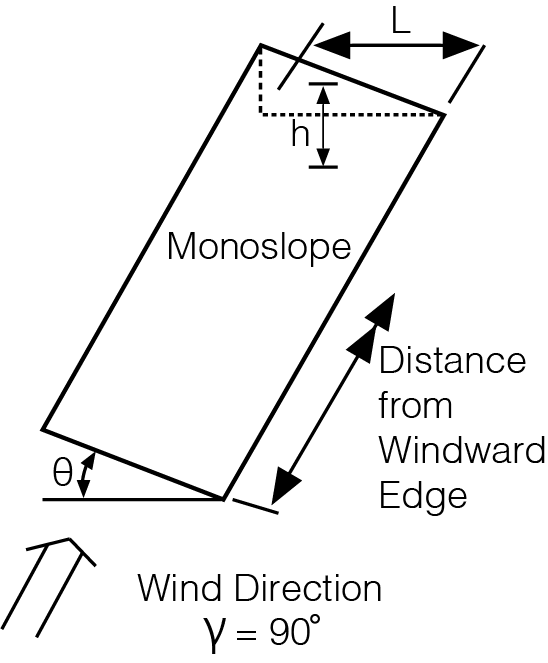
\includegraphics[width=0.300\linewidth]{C:/Users/rodhh/Dropbox/projects/residence_remodel/rivtcalcs0001/docs/d03_models/fig2.png}  \_\_\_\_  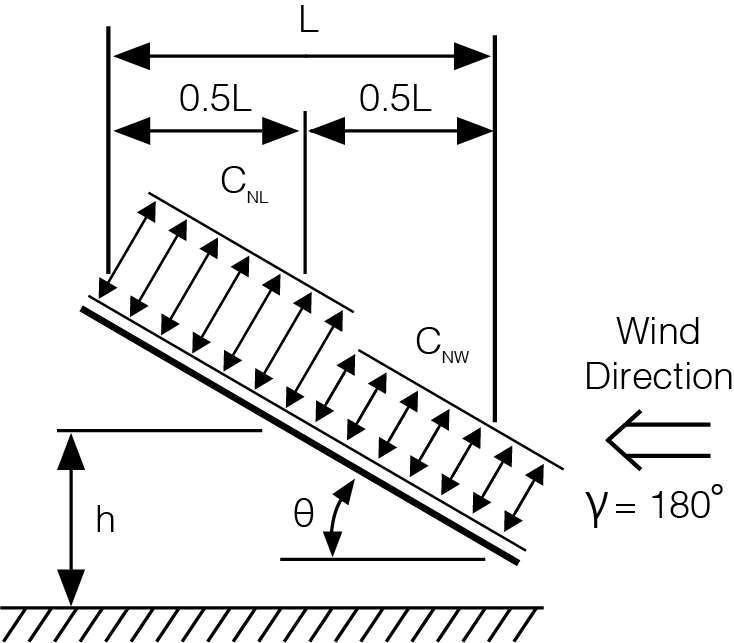
\includegraphics[width=0.400\linewidth]{C:/Users/rodhh/Dropbox/projects/residence_remodel/rivtcalcs0001/docs/d03_models/fig3.png}

\textbf{Wind load geometry - 90 deg} \hfill {[} Fig: 0303.01 {]}

\textbf{Wind load orientation - 180 deg} \hfill {[} Fig: 0303.02 {]}

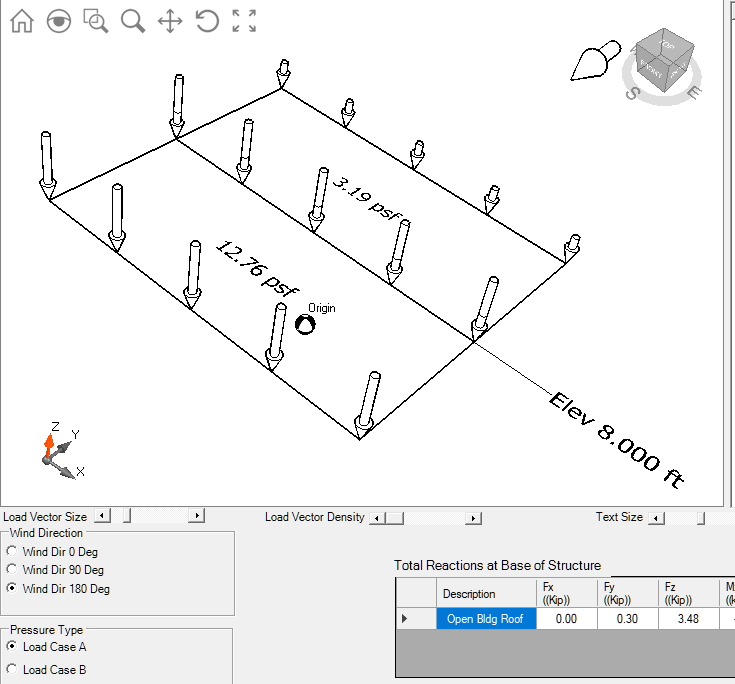
\includegraphics[width=0.450\linewidth]{C:/Users/rodhh/Dropbox/projects/residence_remodel/rivtcalcs0001/docs/d03_models/winda180.png}  \_\_\_\_  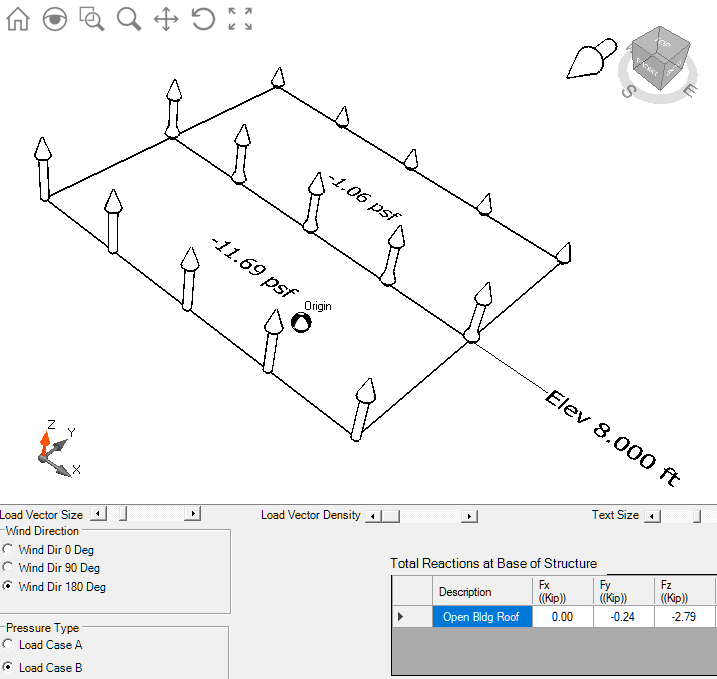
\includegraphics[width=0.450\linewidth]{C:/Users/rodhh/Dropbox/projects/residence_remodel/rivtcalcs0001/docs/d03_models/windb180.png}

\textbf{Positive wind load pressures} \hfill {[} Fig: 0303.03 {]}

\textbf{Negative wind load pressures} \hfill {[} Fig: 0303.04 {]}

\end{document}
